% CS 418: Intro to Data Science — Worksheet 23 (23-week12-day1)
% Week 12, Monday 2026-11-09
% Compile with: latexmk -pdf worksheet.tex

\documentclass[11pt]{article}

% ── Packages ──────────────────────────────────────────────────────────────────
% The wide right margin is the open-ended notes column, half of the 7.2in between the outer margins less a 0.3in gutter; the header and title block span both.
\usepackage[margin=0.65in, right=4.4in, headheight=14pt]{geometry}
\usepackage{amsmath, amssymb}
\usepackage{ragged2e}
% Never break a word across lines, including at hyphens ("Sans-Serif").
\hyphenpenalty=10000
\exhyphenpenalty=10000
\usepackage{enumitem}
\usepackage{booktabs}
\usepackage{graphicx}
\usepackage{hyperref}
\usepackage{xcolor}
\usepackage{fancyhdr}
\usepackage{mdframed}
\usepackage{array}
\usepackage{tabularx}
\usepackage{tikz}

% ── Page style ────────────────────────────────────────────────────────────────
\pagestyle{fancy}
\fancyhf{}
\fancyhfoffset[R]{3.75in}
\lhead{\textbf{CS 418: Intro to Data Science}}
\rhead{UIC, Fall 2026}
\renewcommand{\headrulewidth}{1pt}
\setlength{\headheight}{12pt}
\setlength{\headsep}{0.4cm}

% ── Hyperlinks ────────────────────────────────────────────────────────────────
\hypersetup{colorlinks=false, hidelinks}

% ── Convenience environments ──────────────────────────────────────────────────
% Usage: \fixedblock[height]{content} — a full-width block exactly that tall.
\newcommand{\fixedblock}[2][5.7cm]{\noindent\begin{minipage}[t][#1][t]{\linewidth}\raggedright #2\end{minipage}\par}

% Usage: \vocabrow{term} — one row of checkpoint 3's one-column vocab table: the term in bold, centered vertically by a strut that reaches equally above and below it.
\newcommand{\vocabrow}[1]{\small\textbf{#1}\rule[-0.7em]{0pt}{2.1em}}

% Usage: \sketchbox[width]{height} — a blank box for drawing a graph, half the column wide by default.
\newcommand{\sketchbox}[2][0.5\linewidth]{\framebox[#1]{\rule{0pt}{#2}}}

% Usage: \bridgematrix{A,K,L,V} — an empty 4×4 adjacency matrix, rows and columns labeled, with a separate degree column, for checkpoints 1 and 2.
\newcommand{\bridgematrix}[1]{%
\begin{tikzpicture}[x=0.55cm, y=0.55cm]
  \foreach \l [count=\i] in {#1} {
    \node[font=\scriptsize] at (\i-0.5,4.4) {\l};
    \node[font=\scriptsize] at (-0.4,4.5-\i) {\l};
  }
  \node[font=\scriptsize] at (5.0,4.4) {deg};
  \draw[step=0.55cm] (0,0) grid (4,4);
  \foreach \j in {0,...,3} \draw (4.5,\j) rectangle (5.5,\j+1);
\end{tikzpicture}}

% ══════════════════════════════════════════════════════════════════════════════
\begin{document}
\RaggedRight

% ── Title block: topic left, info box right ───────────────────────────────────
% Spans the notes column too, through the column headings; \makebox lets it run 3.75in past \textwidth without an overfull warning.
\noindent\makebox[\textwidth][l]{\begin{minipage}[t]{\dimexpr\textwidth+3.75in\relax}
\vspace{0pt}
\begin{minipage}[t]{0.55\linewidth}
  \vspace{0pt}
  {\LARGE \textbf{Worksheet \#\,23}} \\[0.18em]
  {\large \textit{Week 12, Day 1: Intro to network analysis}}
\end{minipage}
\hfill
\begin{minipage}[t]{0.40\linewidth}
  \vspace{0pt}
  \small
  Name: \underline{\hspace{4.5cm}} \\[0.35em]
  NetID: \underline{\hspace{4.3cm}} \\[0.35em]
  Date: \underline{\hspace{4.4cm}} \\
\end{minipage}

\vspace{0.6em}
\noindent\rule{\linewidth}{0.6pt}
\vspace{0.1em}

\noindent
\begin{minipage}[t]{3.45in}
  \noindent\underline{\textbf{Guided checkpoints}}\\[0.2em]
  \noindent{\small For full credit, fill in the checkpoints. If you skip a checkpoint, include your own notes for full credit.}
\end{minipage}%
\hspace{0.3in}%
\begin{minipage}[t]{3.45in}
  \noindent\underline{\textbf{Open-ended notes}}\\[0.2em]
\end{minipage}
\end{minipage}}

\vspace{0.8em}

% ── 1. Bridges of Königsberg ─────────────────────────────────────────────────
% Key: nodes A Altstadt, K Kneiphof, L Lomse, V Vorstadt; bridges c, d A–K; g A–L; e K–L; a, b K–V; f L–V. Matrix rows A 0210, K 2012, L 1101, V 0210 (columns A K L V). Degrees A 3, K 5, L 3, V 3: all odd, so no such walk.
\fixedblock[0.33\textheight]{%
\noindent\textbf{1. Bridges of K\"onigsberg}\\[0.18em]
\noindent Draw the graph: one node per land mass, one edge per bridge. Fill in the adjacency matrix (bridges between each pair) and each degree.

\vspace{0.6em}
\noindent\sketchbox{3.8cm}\hfill\bridgematrix{A,K,L,V}

\vspace{0.6em}
\noindent Odd-degree land masses: \underline{\hspace{2.6cm}}
}

\vfill

% ── 2. Bridges of Shikaakwa ──────────────────────────────────────────────────
% Key: bridges a, g, h, i W–N; b, d, e G–N; c, f G–W; j N–L; k W–L. Matrix rows (columns G L N W): G 0032, L 0011, N 3014, W 2140. Degrees G 5, L 2, N 8, W 7. Yes: exactly two land masses (G and W) have odd degree. Euler's rule (§20): more than two odd land masses, impossible; exactly two, possible if the walk starts at one of them; none, possible from anywhere.
\fixedblock[0.42\textheight]{%
\noindent\textbf{2. Bridges of Shikaakwa}\\[0.18em]
\noindent Draw the graph for the bridges on the slide (G Goose Island, L Loop, N North Side, W West Side). Fill in the adjacency matrix and each degree.

\vspace{0.6em}
\noindent\sketchbox{4.2cm}\hfill\bridgematrix{G,L,N,W}

\vspace{0.6em}
\noindent Can one walk cross every bridge exactly once?

\vspace{1.6em}
\noindent What rule(s) did Euler find for when a walk can cross every bridge exactly once?
}

\newpage

% ── 3. Vocab ─────────────────────────────────────────────────────────────────
% Key: definitions from the vocab slides (MMDS Ch. 10; quotes mostly from the summary, Sec. 10.9). A self-loop adds 2 to its node's degree.
\fixedblock[0.28\textheight]{%
\noindent\textbf{3. Vocab}\\[0.18em]
\noindent Write a short definition and/or example for each.

\vspace{0.5em}
\noindent
{\renewcommand{\arraystretch}{1.0}\setlength{\tabcolsep}{4pt}%
\begin{tabular}{|l|}
  \hline
  \vocabrow{Degree}\\ \hline
  \vocabrow{Self-loop}\\ \hline
  \vocabrow{Directed graph}\\ \hline
  \vocabrow{In-degree}\\ \hline
  \vocabrow{Out-degree}\\ \hline
  \vocabrow{Weighted graph}\\ \hline
  \vocabrow{Complete bipartite graph}\\ \hline
\end{tabular}}
}

\vfill

% ── 4. Complete bipartite graph ──────────────────────────────────────────────
% Key: two nodes on one side, three on the other, all six cross edges, none within a side.
\fixedblock[0.22\textheight]{%
\noindent\textbf{4. Complete Bipartite Graph}\\[0.18em]
\noindent Draw the complete bipartite graph $K_{2,3}$.

\vspace{0.4em}
\noindent\sketchbox[\linewidth]{4.2cm}}

\vfill

% ── 5. Triadic closure ───────────────────────────────────────────────────────
% Key: A–D. A and D share two friends (B and C); E–B and E–C share one (A); E–D shares none. Triadic closure: two people with a friend in common are more likely to become friends, and more shared friends make it more likely.
\fixedblock[0.19\textheight]{%
\noindent\textbf{5. Triadic Closure}\\[0.18em]
\noindent In this friendship graph, circle a missing edge most likely to form next. Explain your choice in terms of shared friends.

\vspace{0.4em}
\centering
\begin{tikzpicture}[x=1.0cm, y=0.7cm, every node/.style={circle, draw, thick, minimum size=0.55cm, inner sep=0pt, font=\small}]
  \node (A) at (0,0) {A};
  \node (B) at (1.6,1.3) {B};
  \node (C) at (1.6,-1.3) {C};
  \node (D) at (3.2,0) {D};
  \node (E) at (-1.6,0) {E};
  \draw[thick] (A) -- (B) (A) -- (C) (B) -- (C) (B) -- (D) (C) -- (D) (A) -- (E);
\end{tikzpicture}

\raggedright
}

\vfill

% ── 6. Your project as a network ─────────────────────────────────────────────
% Key: answers vary; e.g., reviewers and restaurants (edge = a review) or agencies and technologies (edge = uses), as on the project slides.
\fixedblock[0.24\textheight]{%
\noindent\textbf{6. Your Project as a Network}\\[0.18em]
\noindent Try to draw a graph from your project's data/concepts.

\vspace{0.4em}
\noindent\sketchbox[\linewidth]{4.2cm}

\vspace{0.4em}
\noindent A node is... \hspace{0.35\linewidth} An edge means...}

\end{document}
